\chapter{Planning}
\label{spec:ch:planning}

To manage the project, the project tool from GitHub will be used.
This allows us to link code with issues that represent activities and add better tracking of the project.
The planning is available on my personal GitHub account~\cite{github-project}.

The following figure \ref{spec:fig:timeline} shows the planning of the project.
On August 4th, the report needs to be finished and sent to the \acrshort{heia} but the internship will continue until the end of August 11th.
Normally, the Bachelor thesis begins directly at the \acrshort{lbl} but due to the time required to get a visa, the plane has been delayed and the project has started in Switzerland.
This week will be used to finish the work on-site and to present the work done to the team.
Exceptionally, the Bachelor's thesis end date can be delayed up to one week due to the disagreement to obtain a visa.

\begin{figure}[ht]
    \centering
    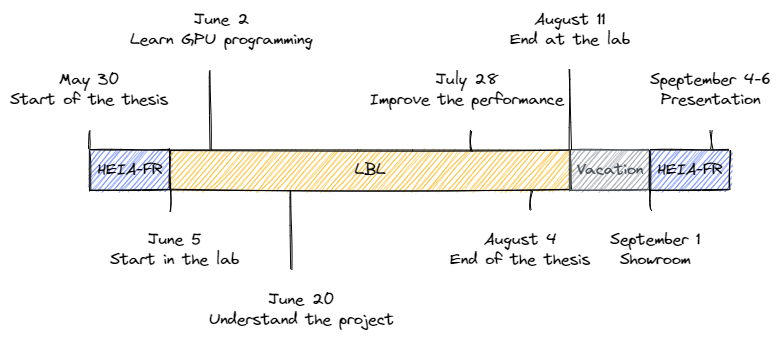
\includegraphics[width=\textwidth]{05-resources/img/spec/planning.excalidraw.png}
    \caption{Timeline of the project}
    \label{spec:fig:timeline}
\end{figure}


On 1st of September, there is a showroom at the \acrshort{heia} where all the students will present their work.
The final presentation will be held between the 4th and the 7th of September.

The detailed planning is available on \href{https://github.com/users/simbarras/projects/3/views/1}{my GitHub} but the figure \ref{spec:fig:planning-gh} is an overview of the planning.

\begin{figure}[ht]
    \centering
    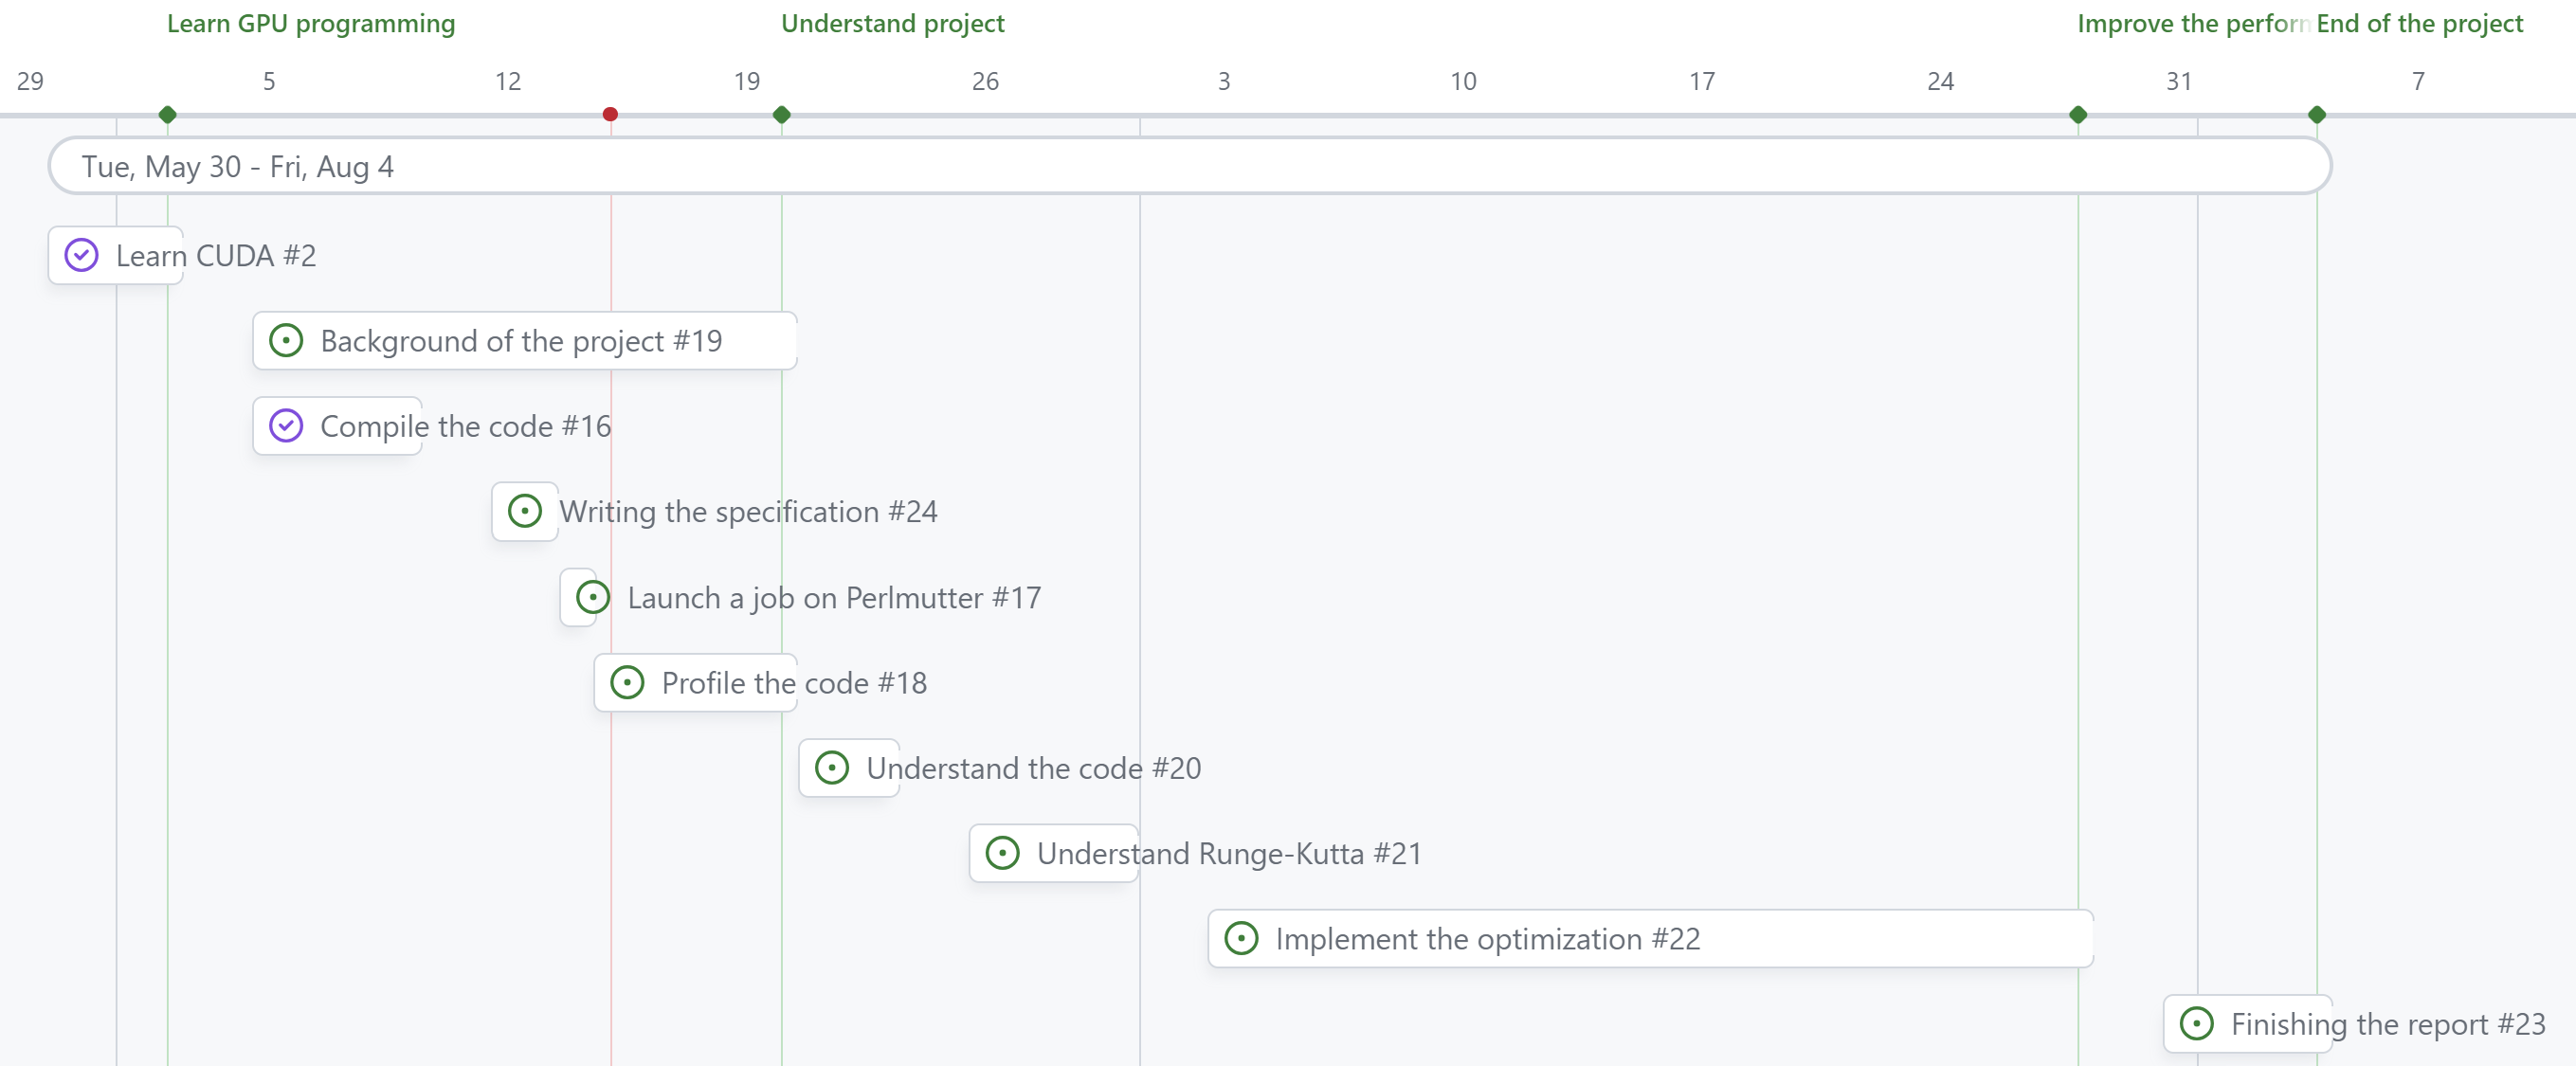
\includegraphics[width=\textwidth]{05-resources/img/spec/planning-gh.png}
    \caption{Planning}
    \label{spec:fig:planning-gh}
\end{figure}


\section{Milestones}
\label{spec:ch:planning:milestones}

The milestones represent the main steps of the project and they are used to track the progress of each step and set a list of activities to do.
The milestones are shown in the project timeline \ref{spec:fig:timeline} and in the GANTT chart \ref{spec:fig:planning-gh} in green.


\section{Issues}
\label{spec:ch:planning:issues}

The issues are representing the tasks that need to be done to complete a milestone.
They can be detailed with a checklist to specify the steps to follow and they can be linked to a pull request to keep a reference to the code that solves the issue.
The GANTT chart \ref{spec:fig:planning-gh} shows the main issues like a Gantt diagram.
